\documentclass{beamer}
\usepackage[utf8]{inputenc}
\usepackage{graphicx}
\usetheme[]{boxes}
\usecolortheme{seagull}
%\usepackage{french}
\title{Modèles et techniques en programmation parallèle hybride et multi-c\oe urs}
\author{Marc Tajchman}\institute{CEA - DEN/DM2S/STMF/LMES}

\begin{document}

\begin{frame}
\titlepage
\end{frame}

\Large
\begin{frame}
  	\frametitle{Plan}
  	\tableofcontents
\end{frame}

\begin{frame}
\section{Rappels sur l'architecture matérielle}
\frametitle{Rappels sur l'architecture matérielle}
On peut voir la structure d'une machine de calcul avec diff\'erents grossissements:
\vfill

Vue globale: un ensemble de n\oe uds de calcul chacun contenant un ou plusieurs processeurs et de la m\'emoire, les n\oe uds sont connect\'e par un r\'eseau:

\vfill
\begin{center}
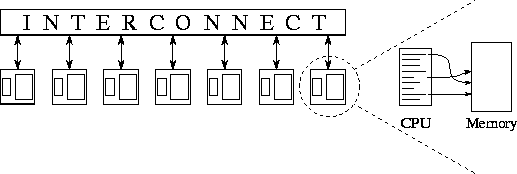
\includegraphics[scale=0.5]{img100}
\end{center}

\vfill
(les machines les plus puissantes actuellement contiennent plusieurs centaines de milliers de n\oe uds)
\end{frame}

\begin{frame}
Vue interne d'un n\oe ud (variable suivant le mod\'ele de processeur et la g\'en\'eration utilis\'ee):

\begin{center}
\includegraphics[scale=0.3]{architecture2}
\end{center}

\end{frame}

\begin{frame}
Vue interne d'un c\oe ur (variable suivant le mod\'ele de processeur et la g\'en\'eration utilis\'ee):

\begin{center}
	\includegraphics[scale=0.3]{architecture2}
\end{center}

\end{frame}

\begin{frame}[fragile]
Situation actuelle (et encore pour plusieurs ann\'ees): 
\begin{quote}
	
	\vfill
	vitesse de calcul (d'un processeur)
	\vfill
	\begin{itemize}
		\item[$\approx$] la m\'emoire interne (registres) du processeur
	        \vfill
	        
		\item[$>$] les diff\'erents m\'emoires interm\'ediaires (caches) entre le processeur et la m\'emoire centrale du n\oe ud (en gris sur la figure pr\'ec\'edente)
			\vfill
			
		\item[$>>$] vitesse de la m\'emoire centrale d'un n\oe ud
			\vfill
			
		\item[$>>$] vitesse du r\'eseau qui connecte les n\oe uds
	\end{itemize}
	\vfill

\end{quote}

\end{frame}

\begin{frame}[fragile]
Fonctionnement :
\begin{enumerate}
	\item Il faut faire voyager les donn\'ees le plus pres possible du processeur qui va les utiliser. 
	\vfill
	
	\item Si une donn\'ee est utilis\'ee $n$ fois par le m\^eme processeur, les $n-1$ derni\'eres utilisations seront plus rapides.
	\vfill
	
	\item Si un processeur a modifi\'e une donn\'ee dans une de ses m\'emoires, il faut r\'epercuter cette modification dans les diff\'erentes copies de cette donn\'ee
	\vfill
\end{enumerate}

Cette gestion utilise du temps d'ex\'ecution (pour assurer la coh\'erence des diff\'erentes parties de la m\'emoire et leurs mises \'a jour correcte.)


\end{frame}

\begin{frame}[fragile]

\bf
\textcolor{blue}{Pour obtenir un code efficace (en temps d'ex\'ecution), il faut:}

\begin{itemize}
	\item utiliser les algorithmes les plus efficaces possible (pas couvert par ce cours)
	
	\item organiser le placement des donn\'ees (am\'eliorer la localit\'e spatiale)
	
	\item organiser la s\'equence d'instruction (am\'eliorer la localit\'e temporelle)

	\item \'ecrire les instructions pour qu'elles soient plus rapides (utilisation du // interne des processeurs)
\end{itemize}
\end{frame}

\begin{frame}
\section{Optimisation de la programmation séquentielle}
\frametitle{Optimisation de la programmation séquentielle \hbox{(2 séances)}}
Points abordés
\begin{itemize}
\item Modèle d'architecture matérielle
\item Localités spatiale et temporelle (optimisation de l'utilisation de la mémoire cache)
\item Parallélisme à l'intérieur d'un c\oe ur
\item Exemples
\end{itemize}
\end{frame}

\begin{frame}
\frametitle{Localité spatiale}
Règle: autant que possible, utiliser des zones mémoires proches les unes des autres dans une séquence d'instructions

\bigskip
But: réduire la fréquence de transferts mémoire centrale - mémoire cache
\end{frame}

\begin{frame}
\frametitle{Localité temporelle}
Règle: autant que possible, pour une zone mémoire, les instructions qui l'utilisent doivent s'exécuter de façon rapprochée

\bigskip
But: réduire la fréquence de transferts mémoire centrale - mémoire cache
\end{frame}

\begin{frame}
\section{Rappels de programmation parallèle}
\subsection{Rappel des notions}
\frametitle{Rappels de programmation parallèle: notions}
Points abordés
\begin{itemize}
\item mémoire distribuée
\item mémoire partagée
\item threads
\item processus
\end{itemize}
\end{frame}

\begin{frame}
\subsection{Mémoire partagée}
\frametitle{Rappels de programmation parallèle: mémoire partagée}
Points abordés
\begin{itemize}
\item Modèle d'architecture matérielle
\item Principes d'optimisation
\item Cas classique : OpenMP, pthreads
\item Autres
\end{itemize}
\end{frame}

\begin{frame}
\subsection{Mémoire distribuée}
\frametitle{Rappels de programmation parallèle: mémoire distribuée}
Points abordés
\begin{itemize}
\item Modèle d'architecture matérielle
\item Principes d'optimisation
\item Cas classique : MPI
\item Autres
\end{itemize}
\end{frame}

\begin{frame}
\section{Programmation parallèle hybride}
\frametitle{Programmation parallèle hybride \hbox{(4 séances)}}
Points abordés
\begin{itemize}
\item Coexistence 
\item Modèles d'hybridation
\item Cas classique : MPI - OpenMP
\item Exemples
\item Autres modèles (e.g. MPI+X, PGAS)
\end{itemize}
\end{frame}

\begin{frame}
\section{Examen}
\frametitle{Examen \hbox{(1 séance)}}
\end{frame}

\end{document}
